\documentclass[conference]{IEEEtran}
\usepackage{amsmath,amssymb}
\usepackage{graphicx}
\usepackage{booktabs}
\usepackage{siunitx}
\usepackage{hyperref}
\usepackage{cite}
\usepackage{bm}

\hypersetup{hidelinks}
\graphicspath{{plots/}}

\title{ADCS Homework 4}
\author{John Zhang}

\begin{document}
\maketitle

% ==================================================================
\section{Actuator Specifications}
\label{sec:actuators}

The ISS uses two classes of ADCS actuators: four large double-gimbal
control moment gyros (CMGs) on the Z1 truss for primary non-propulsive
attitude control, and the Zvezda service-module RCS cluster for
momentum desaturation and reboost.  Public information on the exact
mounting geometry of the CMGs is incomplete, so we model the array as
the standard symmetric 4-CMG pyramid used throughout the
literature~\cite{wie2008,bedrossian2009}, and approximate each CMG as a
single-gimbal unit at the cluster level (which is how the Bedrossian et
al.\ analyses treat them for momentum-envelope and steering-law design).

Both actuator groups are instantiated through the
\texttt{mujoco\_orbit} public API as
\texttt{ControlMomentGyroSpec} and \texttt{ThrusterSpec}, compiled into
\texttt{MjoModel} against \texttt{iss\_model.xml}.  All specifications,
geometry, and Jacobians below are produced by
\texttt{ISS/hw4/actuator\_specs.py}.

The body frame convention is LVLH-aligned at rest: $+X$ along-track
(roll), $+Y$ cross-track (pitch), $+Z$ nadir (yaw).  The
right-handed LVLH attitude used in Sec.~\ref{sec:environmental} places
$+Y_b$ opposite the simulator's positive orbit-normal axis.

% ------------------------------------------------------------------
\subsection{CMG Cluster}
\label{sec:cmg}

\paragraph{Device-level specifications.}  Each CMG is a Honeywell
M1000-class unit with the parameters summarized in
Table~\ref{tab:cmg-specs}~\cite{wie2008,hondatasheet}.  The published
rotor-momentum magnitude is $h = \SI{4760}{N.m.s}$ and the peak output
torque is $\tau_{\max} = \SI{258}{N.m}$; the maximum gimbal rate
follows from these as
$\dot\theta_{\max} = \tau_{\max}/h \approx \SI{0.054}{rad/s}
\approx \SI{3.1}{deg/s}$.

\begin{table}[h]
\centering
\caption{Per-CMG specifications (Honeywell M1000).}
\label{tab:cmg-specs}
\begin{tabular}{@{}lr@{}}
\toprule
Quantity & Value \\
\midrule
Rotor angular momentum $h$          & \SI{4760}{N.m.s} \\
Peak output torque $\tau_{\max}$    & \SI{258}{N.m} \\
Max gimbal rate $\dot\theta_{\max}$ & \SI{0.054}{rad/s} (\SI{3.11}{deg/s}) \\
Gimbal angle range                  & full rotation (wrap-around) \\
\bottomrule
\end{tabular}
\end{table}

\paragraph{Pyramid array geometry.}  Four CMGs are mounted on the Z1
truss with gimbal axes arranged in the standard symmetric pyramid with
skew angle $\beta = \cos^{-1}(1/\sqrt{3}) = 54.7356^\circ$, which
maximizes the inscribed momentum sphere~\cite{wie2008}.  We orient the
pyramid apex along $+Z_\text{body}$.  With azimuths
$\phi_i \in \{0,\; \pi/2,\; \pi,\; 3\pi/2\}$, the gimbal axes
$\hat{\bm g}_i$, the spin axes at neutral gimbal $\hat{\bm s}_i(0)$,
and the output (torque) axes $\hat{\bm t}_i(0) = \hat{\bm g}_i
\times \hat{\bm s}_i(0)$ are listed in
Table~\ref{tab:cmg-geom}.  The neutral spin axes are chosen so that the
net array momentum vanishes at $\bm\theta = \bm 0$:
\begin{equation}
  \bm H(\bm 0) = \sum_{i=1}^{4} h\,\hat{\bm s}_i(0) = \bm 0.
\end{equation}

\begin{table}[h]
\centering
\caption{CMG geometry in the body frame ($\beta = 54.7356^\circ$,
apex $\parallel +Z_\text{body}$).}
\label{tab:cmg-geom}
\small
\setlength{\tabcolsep}{3.5pt}
\begin{tabular}{@{}lccc@{}}
\toprule
CMG & $\hat{\bm g}_i$ & $\hat{\bm s}_i(0)$ & $\hat{\bm t}_i(0)$ \\
\midrule
1 ($\phi = 0$)        & $(+0.816,\;0,\;+0.577)$ & $(0,\;+1,\;0)$ & $(-0.577,\;0,\;+0.816)$ \\
2 ($\phi = \pi/2$)    & $(0,\;+0.816,\;+0.577)$ & $(-1,\;0,\;0)$ & $(0,\;-0.577,\;+0.816)$ \\
3 ($\phi = \pi$)      & $(-0.816,\;0,\;+0.577)$ & $(0,\;-1,\;0)$ & $(+0.577,\;0,\;+0.816)$ \\
4 ($\phi = 3\pi/2$)   & $(0,\;-0.816,\;+0.577)$ & $(+1,\;0,\;0)$ & $(0,\;+0.577,\;+0.816)$ \\
\bottomrule
\end{tabular}
\end{table}

\paragraph{Cluster momentum and Jacobian.}  For an SGCMG at gimbal
angle $\theta_i$, the spin axis in the body frame is
\begin{equation}
  \hat{\bm s}_i(\theta_i) = \cos\theta_i\,\hat{\bm s}_i(0)
    + \sin\theta_i\,\hat{\bm t}_i(0).
\end{equation}
The cluster angular-momentum map and the body-frame torque Jacobian
with respect to commanded gimbal rates $\dot{\bm\theta}\in\mathbb{R}^4$
are therefore
\begin{align}
  \bm H(\bm\theta) &= \sum_{i=1}^{4} h\,\hat{\bm s}_i(\theta_i), \label{eq:cmg-momentum}\\
  A(\bm\theta) &= \frac{\partial \bm\tau_\text{body}}{\partial \dot{\bm\theta}}
                 = -h\,\bigl[\hat{\bm t}_1(\theta_1)\;|\;\hat{\bm t}_2(\theta_2)\;|\;
                             \hat{\bm t}_3(\theta_3)\;|\;\hat{\bm t}_4(\theta_4)\bigr], \label{eq:cmg-jacobian}
\end{align}
where $\hat{\bm t}_i(\theta_i) = \hat{\bm g}_i \times \hat{\bm s}_i(\theta_i)$.
The negative sign in~\eqref{eq:cmg-jacobian} comes from Newton's third
law: the body torque is the reaction to
$\mathrm{d}\bm h_i^\text{body}/\mathrm{d}t
= h\,\dot\theta_i\,\hat{\bm t}_i$.

Evaluated at the neutral gimbal state $\bm\theta = \bm 0$,
\begin{equation}
  A(\bm 0) = \begin{bmatrix}
      +2748 &  0      & -2748 &  0 \\
      0     & +2748   & 0     & -2748 \\
      -3887 & -3887   & -3887 & -3887
  \end{bmatrix}\ \si{N.m \per rad \per s}.
  \label{eq:A0}
\end{equation}
Rows 1 and 2 have the sparsity pattern
$\pm h\cos\beta\cdot\hat{\bm s}_i^{xy}$ (only opposing-azimuth CMGs
contribute to roll/pitch torque at $\bm\theta = \bm 0$), and the
row-3 entries are all $-h\sin\beta = -3887$~N$\cdot$m per rad/s, so all
four CMGs contribute constructively to yaw torque in the zero-gimbal
configuration.  This is a well-known feature of the pyramid array and
is why the "null motion" direction at $\bm\theta = \bm 0$
($\dot{\bm\theta} = (1,1,1,1)$) produces a pure $-Z$ torque of
magnitude $4h\sin\beta\cdot\dot\theta_{\max} \approx \SI{842}{N.m}$.

\paragraph{Momentum envelope.}  Sampling $\bm\theta\in[-\pi,\pi]^4$
uniformly and plotting $\bm H(\bm\theta)$ gives the solid region
shown in Fig.~\ref{fig:cmg-envelope}.  Its maximum extent is
$4h = \SI{19040}{N.m.s}$ (when all spin axes align), and the largest
inscribed sphere has radius $2h\cos(\beta/2) \approx
\SI{8454}{N.m.s}$.

\begin{figure}[h]
\centering
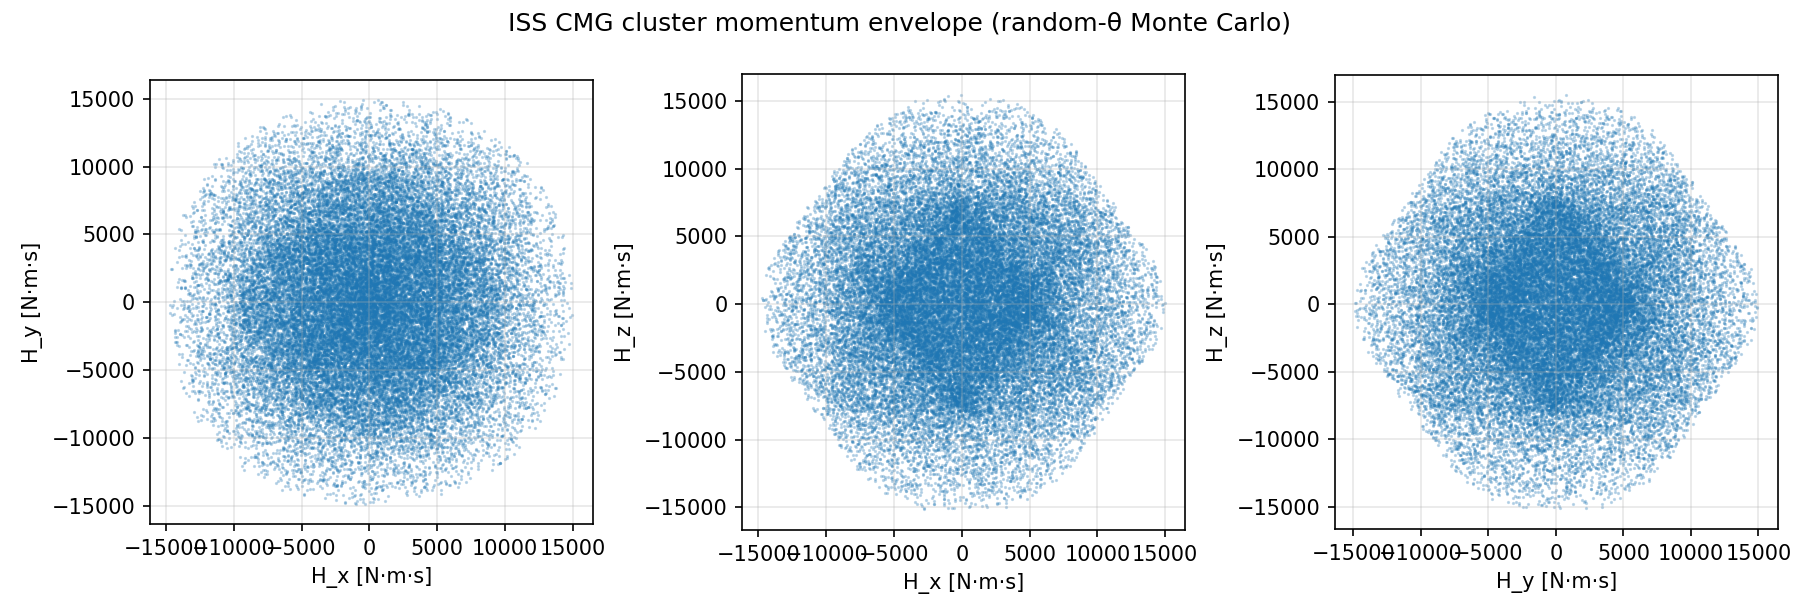
\includegraphics[width=\linewidth]{cmg_momentum_envelope.png}
\caption{Cluster angular-momentum envelope of the 4-CMG pyramid
($40\,000$ random gimbal configurations).  Projections on the three
body-frame coordinate planes.  The envelope is convex in each
projection; internal singular surfaces exist within the solid region
(not shown).}
\label{fig:cmg-envelope}
\end{figure}

\paragraph{Output-torque set.}  At $\bm\theta = \bm 0$, the image of
the unit $\dot{\bm\theta}$-ball under $A(\bm 0)$, scaled by
$\dot\theta_{\max}$, is the rank-3 ellipsoid of body torques
simultaneously achievable without saturating any gimbal
(Fig.~\ref{fig:cmg-torque}).  The ellipsoid is stretched along $\pm Z$
because row~3 of~\eqref{eq:A0} is coherent across all four CMGs.

\begin{figure}[h]
\centering
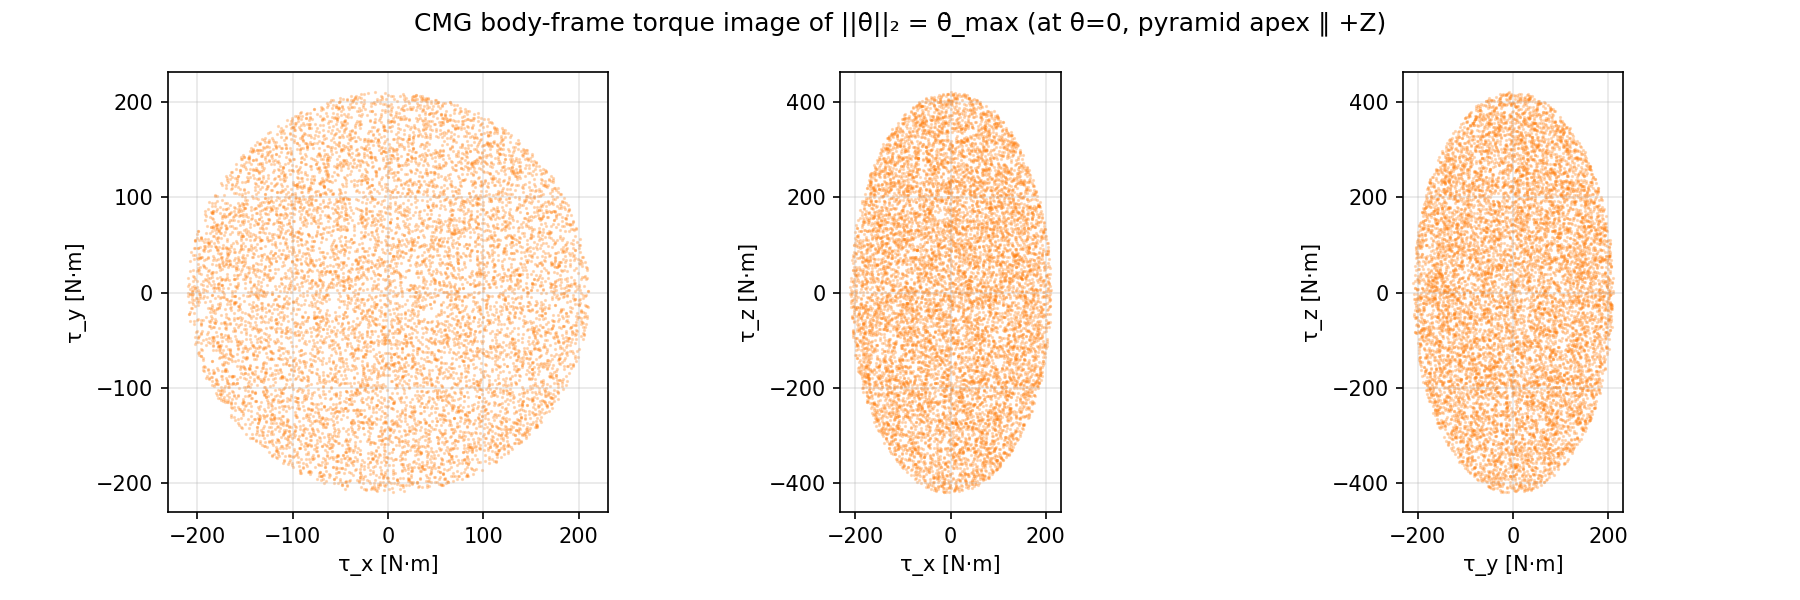
\includegraphics[width=\linewidth]{cmg_torque_image.png}
\caption{Image of $\|\dot{\bm\theta}\|_2 = \dot\theta_{\max}$ under
$A(\bm 0)$ — the body-frame torques reachable without exceeding any
gimbal-rate limit at the zero-gimbal configuration.}
\label{fig:cmg-torque}
\end{figure}

% ------------------------------------------------------------------
\subsection{Zvezda RCS Thrusters}
\label{sec:thrusters}

The Russian Zvezda service module provides the ISS's only on-station
propulsive ADCS authority.  Its aft propulsion assembly (PAO) houses
$\sim$32 small DPO attitude thrusters (\SI{130}{N}
class)~\cite{nasa_iss_prop} and 2 large DKD reboost engines
(\SI{3070}{N} class).  For this analysis we use a simplified symmetric
layout of 8 attitude thrusters on the aft rings plus the 2 aft-facing
reboost engines (Table~\ref{tab:thrusters}).  Positions are given with
respect to the ISS center of mass, which is approximately
\SI{30}{m} forward of Zvezda's aft bulkhead.

\begin{table*}[h]
\centering
\caption{Simplified Zvezda RCS layout modeled in \texttt{actuator\_specs.py}.}
\label{tab:thrusters}
\small
\begin{tabular}{@{}llccc@{}}
\toprule
Role & Label & Position [m] & Direction & $F_{\max}$ [N] \\
\midrule
Attitude (ring, top/bot ±Y)    & ACS\_+Y\_top & $(-30,+3,+3)$ & $(0,+1,0)$ & 130 \\
                               & ACS\_-Y\_top & $(-30,-3,+3)$ & $(0,-1,0)$ & 130 \\
                               & ACS\_+Y\_bot & $(-30,+3,-3)$ & $(0,+1,0)$ & 130 \\
                               & ACS\_-Y\_bot & $(-30,-3,-3)$ & $(0,-1,0)$ & 130 \\
Attitude (ring, fwd/aft ±Z)    & ACS\_+Z\_fwd & $(-29,0,+3)$  & $(0,0,+1)$ & 130 \\
                               & ACS\_+Z\_aft & $(-31,0,+3)$  & $(0,0,+1)$ & 130 \\
                               & ACS\_-Z\_fwd & $(-29,0,-3)$  & $(0,0,-1)$ & 130 \\
                               & ACS\_-Z\_aft & $(-31,0,-3)$  & $(0,0,-1)$ & 130 \\
Reboost (DKD)                  & DKD\_stbd    & $(-31.5,+0.8,0)$ & $(+1,0,0)$ & 3070 \\
                               & DKD\_port    & $(-31.5,-0.8,0)$ & $(+1,0,0)$ & 3070 \\
\bottomrule
\end{tabular}
\end{table*}

\paragraph{Wrench Jacobian.}  Each thruster produces a body-frame
force $\hat{\bm d}_i F_i$ and a torque $\bm r_i \times \hat{\bm d}_i F_i$
about the CM, so the full $6\times N$ wrench Jacobian is
\begin{equation}
  B = \begin{bmatrix} \hat{\bm d}_1 & \cdots & \hat{\bm d}_N \\
                      \bm r_1 \times \hat{\bm d}_1 & \cdots & \bm r_N \times \hat{\bm d}_N
        \end{bmatrix},
  \qquad \begin{bmatrix}\bm F \\ \bm \tau\end{bmatrix}_\text{body} = B\,\bm u,
  \label{eq:thr-B}
\end{equation}
with $\bm u \in [0, F_{\max,i}]^N$.  The numerical evaluation gives
\begin{equation}
\resizebox{\columnwidth}{!}{$\displaystyle
  B = \left[\begin{array}{cccccccccc}
    0 & 0 & 0 & 0 & 0 & 0 & 0 & 0 & +1 & +1 \\
    +1 & -1 & +1 & -1 & 0 & 0 & 0 & 0 & 0 & 0 \\
    0 & 0 & 0 & 0 & +1 & +1 & -1 & -1 & 0 & 0 \\
    -3 & +3 & +3 & -3 & 0 & 0 & 0 & 0 & 0 & 0 \\
    0 & 0 & 0 & 0 & +29 & +31 & -29 & -31 & 0 & 0 \\
    -30 & +30 & -30 & +30 & 0 & 0 & 0 & 0 & -0.8 & +0.8
  \end{array}\right].
  $}
  \label{eq:B-num}
\end{equation}
The top three rows give body-frame force per unit thrust and the bottom
three give torque per unit thrust.  Firing each pair of Y-thrusters in
the same direction produces a pure roll or yaw couple; firing each
Z-pair in the same direction produces a pure pitch couple; the two DKD
engines provide pure along-track force (with a small residual yaw
couple from their $\pm Y$ lever arms).

\paragraph{Maximum body wrenches.}  Saturating the thrusters that
contribute in a given axis direction gives the upper-bound pure-torque
capabilities in Table~\ref{tab:thr-capacity}.  Roll authority is the
weakest (limited to the $\pm 3$\,m ring radius), while yaw authority is
the strongest (benefiting from the $\sim 30$\,m lever arm along $-X$).

\begin{table}[h]
\centering
\caption{Upper-bound pure-torque and reboost capabilities from the
simplified Zvezda layout.}
\label{tab:thr-capacity}
\begin{tabular}{@{}lc@{}}
\toprule
Command & Max magnitude \\
\midrule
Pure roll torque $\tau_x$     & \SI{780}{N.m}  \\
Pure pitch torque $\tau_y$    & \SI{7800}{N.m} \\
Pure yaw torque $\tau_z$      & \SI{10256}{N.m} \\
Pure $+X$ force (reboost)     & \SI{6140}{N}  \\
\bottomrule
\end{tabular}
\end{table}

\paragraph{Use in the overall ADCS.}  Although the thrusters have much
higher instantaneous torque than the CMG cluster, they are
propellant-limited and are not used for continuous attitude regulation.
Their role is to perform CMG desaturation (momentum dumping) when
secular disturbance torques accumulate to the cluster momentum limit,
and to execute orbit reboost.  Quantitative estimates of how often
desaturation is required are addressed in
Sec.~\ref{sec:environmental}.

% ==================================================================
\section{Environmental Torques}
\label{sec:environmental}

For HW4 Q2 I added gravity-gradient torque and aerodynamic drag to the
single-rigid-body ISS model.  Drag is the appropriate surface-force
perturbation for this orbit: at \SI{408}{km}, the atmosphere model gives
$\rho=\SI{2.28e-13}{kg.m^{-3}}$ and
$v=\SI{7.66}{km/s}$, so
$q=\frac12\rho v^2=\SI{6.71e-6}{N.m^{-2}}$.  With $C_D=2.2$ the
effective drag pressure is \SI{1.48e-5}{N.m^{-2}}, larger than a
representative solar-radiation pressure load
($1.8P_\odot=\SI{8.21e-6}{N.m^{-2}}$).  Drag also acts continuously in
LEO and changes the orbit energy, so it is the more relevant choice for
the ISS than SRP.

All Q2 data are generated by
\texttt{ISS/hw4/environmental\_torques.py}.  The script uses
\[
  J=\mathrm{diag}(128,\;107,\;201)\times 10^6\ \si{kg.m^2},
\]
the HW2 flat-plate ISS surface model, and a circular \SI{408}{km},
$51.6^\circ$ orbit with period \SI{92.72}{min}.  The simulator LVLH
axes are $+x$ radial-out, $+y$ along-track, and $+z$ orbit-normal.  The
right-handed nominal ISS attitude used here is computed as
\[
  +X_b \parallel +y_\text{LVLH}, \qquad
  +Z_b \parallel -x_\text{LVLH}, \qquad
  +Y_b \parallel -z_\text{LVLH}.
\]
This is the ``nominal alignment'' used in the plots and tables.

\subsection{Torque Models}

For each rigid body, the gravity-gradient torque is
\begin{equation}
  \bm\tau_\text{gg}
    = \frac{3\mu}{r^3}\,\hat{\bm r}\times
      \left(J\hat{\bm r}\right),
  \label{eq:gg-torque}
\end{equation}
where $\hat{\bm r}$ and $J$ are expressed in the same frame.  The code
rotates MuJoCo's principal-axis inertia into the world/LVLH frame using
\texttt{ximat}, so non-diagonal \texttt{fullinertia} models are handled
correctly.  This is the missing term for a large spacecraft modeled as
one rigid body; point gravity at the body COM cannot generate this
rotational torque.

Drag is applied to each flat plate as
\begin{equation}
  \bm F_D
    = -\frac12 \rho C_D A_\text{proj}
      \|\bm v_\text{rel}\|\,\bm v_\text{rel},
  \qquad
  \bm\tau_D = \bm r_\text{cp}\times\bm F_D ,
  \label{eq:drag-torque}
\end{equation}
where $\bm v_\text{rel}$ includes atmospheric co-rotation.

\subsection{Experiment Design}

The homework asks for free simulations over several orbits, so the main
experiment is a three-orbit uncontrolled response with four perturbation
sets: none, gravity gradient only, drag only, and both.  I run that
experiment from two initial attitudes:
\begin{itemize}
  \item exact nominal LVLH/nadir alignment; and
  \item an off-nominal body-axis offset of
        $(5^\circ,-3^\circ,2^\circ)$, whose total attitude error is
        \SI{6.12}{deg}.
\end{itemize}
The second initial condition is not a hidden controller assumption; it
is a stated perturbation that makes the gravity-gradient dynamics
visible.  Separately, I compute fixed-reference torque histories over
one day.  Those histories estimate how much angular momentum the CMGs
would accumulate if an attitude controller were holding a commanded
attitude.

\subsection{Torque Magnitudes}

The nominal LVLH attitude has zero gravity-gradient torque because the
radial direction is exactly the principal $-Z_b$ axis:
$\hat{\bm r}\times J\hat{\bm r}=0$.  This is why the gravity-gradient
bar is effectively absent in the nominal case.  When the spacecraft is
started from the stated off-nominal attitude, gravity gradient is the
dominant torque.  The analytical all-attitude upper bound is
\[
  \tau_{\text{gg,max}}
  = \frac{3\mu}{2r^3}\left(I_{\max}-I_{\min}\right)
  = \SI{179.84}{N.m}.
\]

\begin{table}[h]
\centering
\caption{Fixed-reference environmental torques used for sizing.}
\label{tab:env-torques}
\begin{tabular}{@{}lcc@{}}
\toprule
Reference attitude & Max $\|\bm\tau\|$ & Orbit-avg. $\|\bar{\bm\tau}\|$ \\
\midrule
Nominal GG       & $\approx 0$ & $\approx 0$ \\
Nominal drag     & \SI{6.11e-3}{N.m} & \SI{2.79e-4}{N.m} \\
Offset GG        & \SI{34.32}{N.m} & \SI{34.25}{N.m} \\
Offset drag      & \SI{9.12e-3}{N.m} & \SI{5.83e-3}{N.m} \\
\bottomrule
\end{tabular}
\end{table}

\begin{figure}[h]
\centering
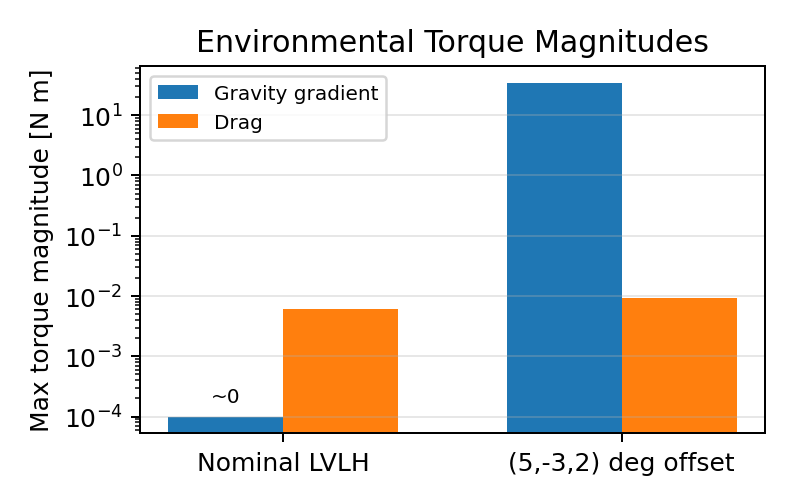
\includegraphics[width=\linewidth]{environmental_torque_magnitude.png}
\caption{Maximum fixed-reference torque magnitudes.  The nominal
gravity-gradient value is numerical roundoff because the radial
direction is a principal inertia axis.}
\label{fig:env-torque}
\end{figure}

\subsection{Orbit Averages and Momentum Accumulation}

For the nominal LVLH reference attitude, gravity gradient contributes no
secular momentum.  The drag orbit-average is
\[
  \bar{\bm\tau}_D =
  (-8.23\times10^{-8},\;-5.16\times10^{-6},\;2.79\times10^{-4})
  \ \si{N.m},
\]
which gives \SI{28.5}{N.m.s} maximum accumulated momentum over one day
in the time-domain integration.  The orbit-average estimate gives
\SI{24.1}{N.m.s/day}.  Both are tiny compared with the
\SI{8454}{N.m.s} conservative CMG inscribed momentum radius.

The off-nominal fixed-reference case is different: holding the
$(5^\circ,-3^\circ,2^\circ)$ attitude offset against gravity gradient
would accumulate \SI{2.96e6}{N.m.s} in one day and would fill the
conservative CMG envelope in about \SI{4.1}{min}.  This is a sizing
warning, not the expected operating mode.

\begin{figure}[h]
\centering
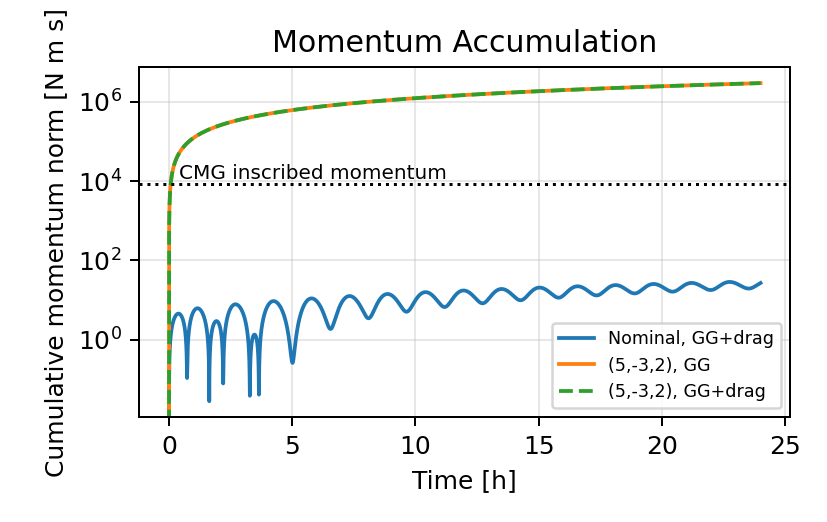
\includegraphics[width=\linewidth]{environmental_momentum_accumulation.png}
\caption{Cumulative momentum required to reject the modeled
disturbances.  The nominal case is drag-limited; the offset reference is
gravity-gradient dominated, so the gravity-gradient-only and combined
curves nearly overlap.}
\label{fig:env-momentum}
\end{figure}

\subsection{Several-Orbit Free Response}

Figure~\ref{fig:env-attitude} shows the free attitude simulations.  From
exact nominal LVLH, the no-perturbation and gravity-gradient-only cases
remain fixed because the initial attitude is an equilibrium.  Drag alone
causes only \SI{0.011}{deg} drift over three orbits.  With drag and
gravity gradient together, drag first pushes the body away from the
exact equilibrium and gravity gradient then dominates the rotational
motion, reaching about \SI{180}{deg} error and
\SI{9.76e-2}{deg/s}.

From the off-nominal initial attitude, the no-perturbation case stays at
the initial \SI{6.12}{deg} error.  Drag alone changes that by only
\SI{0.38}{deg}.  Gravity gradient drives the main free response, with
maximum rate \SI{1.01e-1}{deg/s}.  The added drag barely changes the curve
because the off-nominal gravity-gradient torque is about four orders of
magnitude larger than the drag torque.

\begin{figure}[h]
\centering
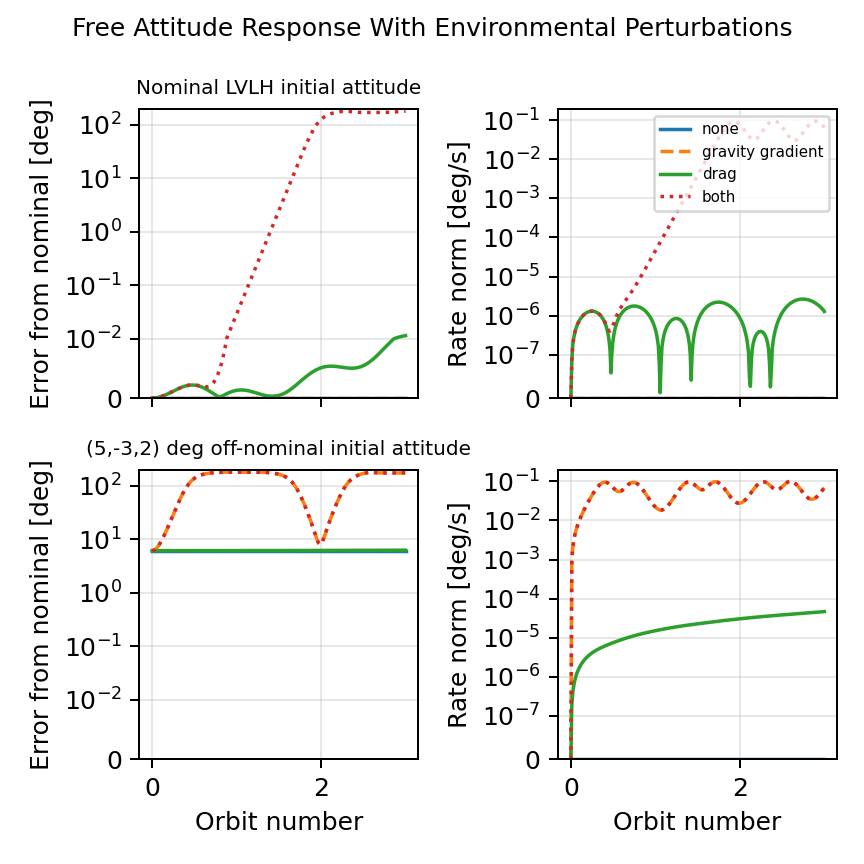
\includegraphics[width=\linewidth]{environmental_attitude_response.png}
\caption{Uncontrolled three-orbit attitude response with and without
each perturbation.  The ordinate uses a symmetric-log scale so the small
drag response and the large gravity-gradient response are both visible.}
\label{fig:env-attitude}
\end{figure}

\subsection{ADCS Implications}

The CMG cluster has ample instantaneous torque authority for these
modeled disturbances: even the off-nominal \SI{34.32}{N.m}
gravity-gradient torque is well below the hundreds of \si{N.m}
available from the CMGs.  The main issue is momentum management and
attitude stability.  In nominal LVLH, the modeled drag load would fill
the conservative CMG momentum sphere only after roughly
\SIrange{300}{350}{days}, depending on whether the one-day peak or the
orbit-averaged secular value is used.  Real ISS desaturation will be
driven by additional unmodeled biases and operational constraints, but
this model does not predict frequent momentum dumping from drag alone.

Gravity gradient is not a nominal momentum-dumping driver when the ISS
is aligned with LVLH because its torque is zero at that equilibrium.
It is still important for the nonlinear attitude simulation: once the
vehicle is a few degrees away from the principal-axis alignment, the
gravity-gradient torque dominates the free response and must be included
in the controller test cases for Q3.

% ==================================================================
\section{Attitude Regulation}
\label{sec:regulation}

For Q3 I designed a continuous-time linear-quadratic regulator (LQR)
to hold the same earth-pointing LVLH attitude used in
Sec.~\ref{sec:environmental}.  The controller state is
\[
  \bm x =
  \begin{bmatrix}
    \delta\bm\theta^\top & \bm\omega^\top
  \end{bmatrix}^\top ,
\]
where $\delta\bm\theta$ is the small attitude-error rotation vector
from the nominal LVLH attitude and $\bm\omega$ is the body angular
velocity relative to the LVLH frame, expressed in the body frame.  The
linearized torque-input model is
\begin{equation}
  \dot{\bm x}
  =
  \begin{bmatrix}
    0_{3\times3} & I_3 \\
    0_{3\times3} & 0_{3\times3}
  \end{bmatrix}\bm x
  +
  \begin{bmatrix}
    0_{3\times3} \\
    J^{-1}
  \end{bmatrix}\bm\tau .
  \label{eq:lqr-linearization}
\end{equation}
I used Bryson-style weights corresponding to
\SI{30}{deg} attitude error, \SI{0.05}{deg/s} rate error, and
\SI{250}{N.m} control torque.  Solving the continuous algebraic
Riccati equation gives the body-frame control law
\[
  \bm\tau_c = -K\bm x,
\]
with the diagonal gains in Table~\ref{tab:lqr-gains}.  Commands are
limited to $(300,300,700)$~N$\cdot$m in body roll, pitch, and yaw and
then mapped to the four-CMG pyramid using the least-norm gimbal-rate
solution
\[
  \dot{\bm\theta}_g = A(\bm\theta_g)^\dagger\bm\tau_c ,
\]
with the gimbal-rate limit from Sec.~\ref{sec:cmg}.

\begin{table}[h]
\centering
\caption{LQR gains for $\bm\tau_c=-K[\delta\bm\theta^\top,\bm\omega^\top]^\top$.}
\label{tab:lqr-gains}
\begin{tabular}{@{}lcc@{}}
\toprule
Axis & $K_\theta$ [N m/rad] & $K_\omega$ [N m s/rad] \\
\midrule
Roll  & 477.5 & $4.52\times10^5$ \\
Pitch & 477.5 & $4.29\times10^5$ \\
Yaw   & 477.5 & $5.23\times10^5$ \\
\bottomrule
\end{tabular}
\end{table}

\subsection{Perfect-State Initial-Condition Tests}

The first test uses perfect state feedback and no environmental
disturbances, so it isolates the nonlinear attitude-regulation
behavior from estimator and disturbance effects.  I generated eight
random attitude errors with magnitudes from $15^\circ$ to $90^\circ$
and small initial body rates.  All cases converged to the nominal
earth-pointing attitude within two orbits.  The worst settling time to
remain below \SI{0.1}{deg} attitude error and
\SI{0.01}{deg/s} rate was \SI{8800}{s} (\SI{1.58}{orbits}), and the
largest final attitude error was \SI{0.017}{deg}.  The largest
achieved CMG torque was \SI{479}{N.m}.

\begin{figure}[h]
\centering
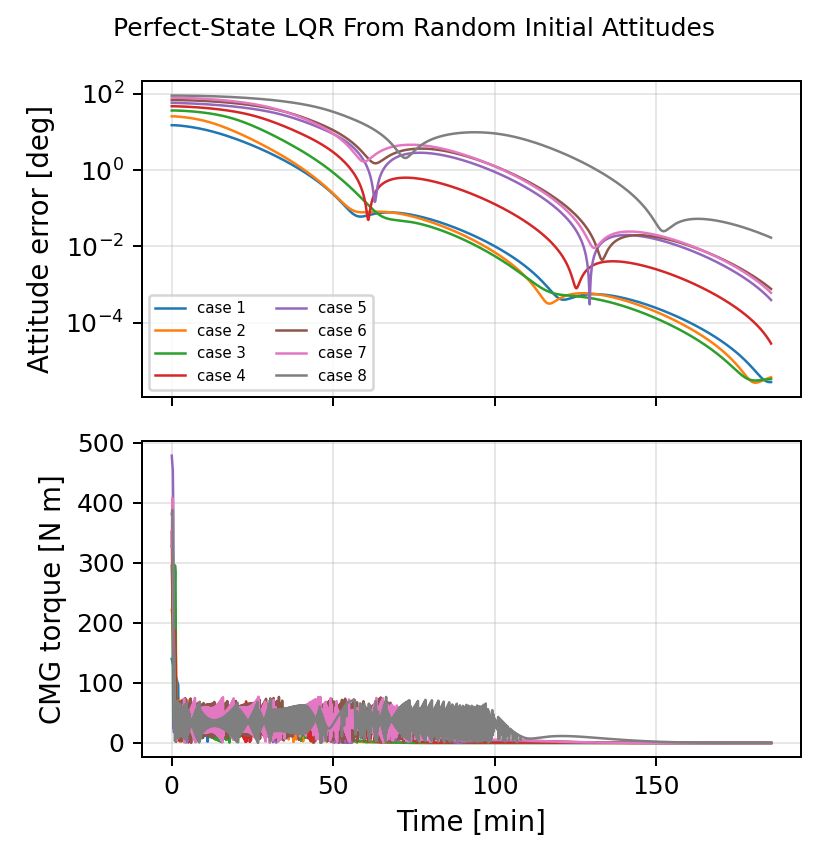
\includegraphics[width=\linewidth]{attitude_regulation_random_ic.png}
\caption{Perfect-state LQR response from eight random initial attitude
errors up to $90^\circ$.  The CMGs saturate briefly for the largest
slews, but all cases settle within the two-orbit simulation window.}
\label{fig:lqr-random}
\end{figure}

\subsection{Disturbed Orbit With Perfect State}

Next I enabled gravity gradient and drag and initialized the spacecraft
at $(2^\circ,-1^\circ,1^\circ)$ from the nominal earth-pointing
attitude.  With perfect state feedback, the three-orbit simulation had
a final attitude error of \SI{0.027}{deg}.  The RMS nadir-pointing
error over the last orbit was \SI{0.070}{deg}, and the maximum
controller torque was only \SI{20.4}{N.m}.  This shows that once the
large initial error is removed, the LQR torque needed to reject the Q2
environmental disturbances is small compared with CMG authority.

\begin{figure}[h]
\centering
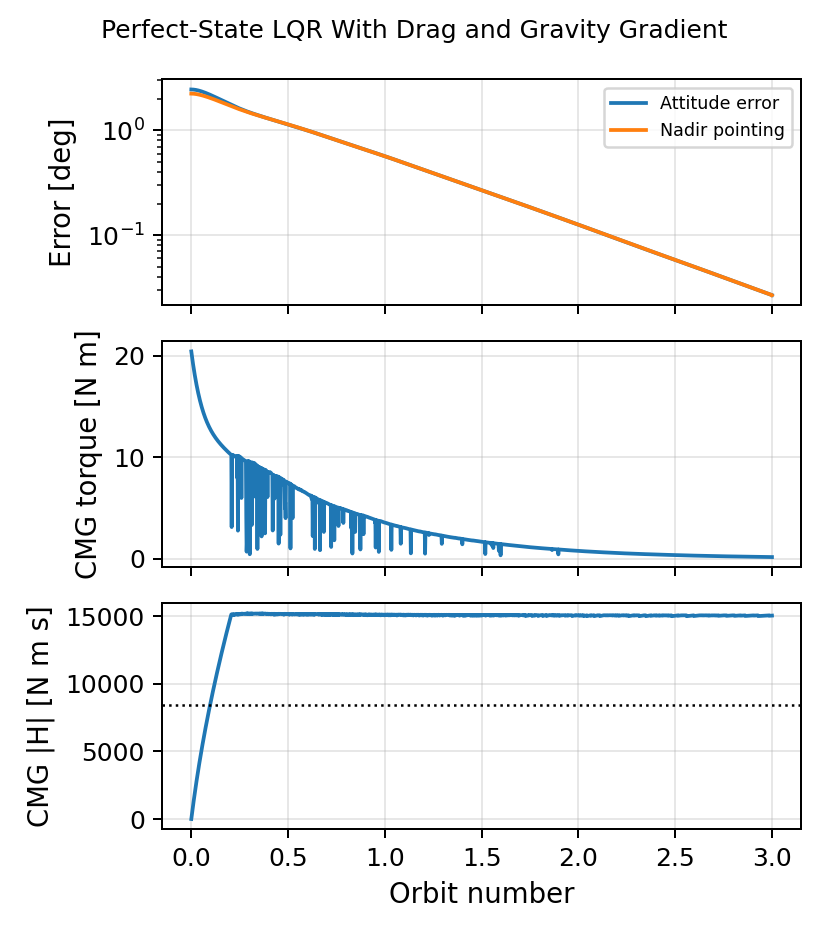
\includegraphics[width=\linewidth]{attitude_regulation_disturbed.png}
\caption{Perfect-state LQR hold with gravity-gradient torque and drag
enabled.  The bottom panel shows the simple CMG steering law's stored
momentum; no momentum-management null motion or desaturation is added
in this controller baseline.}
\label{fig:lqr-disturbed}
\end{figure}

\subsection{HW3 Estimator in the Loop}

Finally, I replaced the perfect attitude and rate state with the HW3
MEKF estimate.  The truth simulation uses the HW3 gyro random-walk
model, star-tracker quaternion measurements, and magnetometer, sun, and
horizon vector measurements.  The controller receives the MEKF
ECI-frame attitude estimate, converts it to the current LVLH frame, and
subtracts the LVLH frame rate from the bias-corrected gyro measurement
before applying the same LQR gain.

The estimator-in-the-loop case remains stable for the same three-orbit
disturbed simulation.  The last-orbit RMS nadir-pointing error is
\SI{0.092}{deg}; the last-orbit RMS MEKF attitude error is
\SI{0.0061}{deg}, with a maximum estimator attitude error of
\SI{0.018}{deg}.  The sensor noise therefore increases pointing error
only slightly relative to the perfect-state baseline for this
disturbance level.

\begin{figure}[h]
\centering
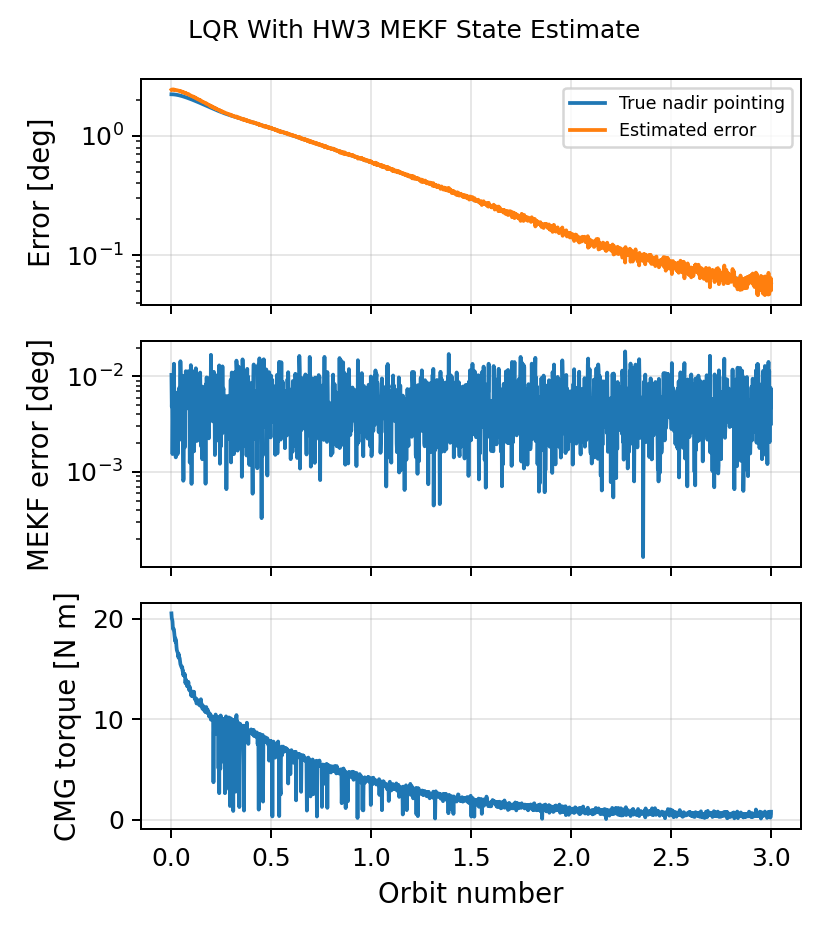
\includegraphics[width=\linewidth]{attitude_regulation_estimator.png}
\caption{LQR attitude hold using the HW3 MEKF state estimate.  The
estimated control error tracks the true nadir-pointing error closely;
the middle panel shows the MEKF attitude error relative to truth.}
\label{fig:lqr-estimator}
\end{figure}

\paragraph{Limitations.}  The CMG steering law used here is a
least-norm torque map, not a full ISS singularity-avoidance or
momentum-management steering law.  Large initial slews drive the modeled
CMG momentum above the conservative inscribed sphere, although still
inside the sampled full momentum envelope from Sec.~\ref{sec:cmg}.  A
flight-quality implementation would add null-motion steering and
periodic desaturation with the RCS; this is separate from the LQR state
feedback design tested here.

% ==================================================================
\section{Eigen-Axis Slew}
\label{sec:slew}

For Q4 I implemented an eigen-axis slew planner in
\texttt{ISS/hw4/eigen\_axis\_slew.py}.  The planner follows the
Lecture~16 construction~\cite{manchester_l16}: compute the relative
attitude
\[
  R_e = R_0^\top R_f = \exp(\phi_f \hat{\bm e}^{\times}),
\]
then move from the initial attitude $R_0$ to the final attitude $R_f$
by
\begin{equation}
  R(t) = R_0 \exp(\phi(t)\hat{\bm e}^{\times}).
  \label{eq:eigen-axis-path}
\end{equation}
I used the versine rest-to-rest profile
\begin{equation}
  \phi(t) = \frac{\phi_f}{2}\left(1-\cos\frac{\pi t}{T}\right),
  \qquad 0 \le t \le T ,
  \label{eq:versine}
\end{equation}
with $\dot\phi(0)=\dot\phi(T)=0$.  The nominal body-frame angular
velocity and acceleration are therefore
\[
  \bm\omega_d = \dot\phi\,\hat{\bm e}, \qquad
  \dot{\bm\omega}_d = \ddot\phi\,\hat{\bm e}.
\]
The inverse-dynamics feedforward torque is the rigid-body Euler torque
\begin{equation}
  \bm\tau_\text{ff}
  = J\dot{\bm\omega}_d
    + \bm\omega_d\times J\bm\omega_d .
  \label{eq:slew-inv-dyn}
\end{equation}

\subsection{Actuator Choice and Tracking Law}

The requested test is a $180^\circ$ maneuver.  I chose an initial
attitude that is $180^\circ$ away from the nominal LVLH earth-pointing
attitude by a pitch-axis flip, then slewed back to the nominal
attitude.  The resulting eigen-axis in the initial body frame is
$-\hat{\bm y}_b$.  With a one-orbit maneuver time
$T=\SI{5563}{s}=\SI{92.72}{min}$, the nominal maximum rate is
\SI{0.0508}{deg/s} and the inverse-dynamics torque peaks at only
\SI{53.6}{N.m}.

Peak torque alone is not the limiting actuator constraint.  The same
one-orbit maneuver requires
\[
  \max_t \|J\bm\omega_d(t)\| = \SI{9.49e4}{N.m.s}
\]
of spacecraft angular momentum, which is much larger than both the
sampled CMG full envelope from Sec.~\ref{sec:cmg}
($4h=\SI{1.904e4}{N.m.s}$) and the conservative inscribed sphere
($\SI{8454}{N.m.s}$).  A CMG-only one-orbit $180^\circ$ slew would
therefore violate the momentum capability even though the torque demand
looks small.  For this Q4 test I used the Zvezda RCS attitude-thruster
couples from Sec.~\ref{sec:thrusters}, keeping each thruster below its
\SI{130}{N} limit and strongly penalizing net force in the allocator.

The tracking controller uses the Q3 LQR gain, scaled by a factor of
two, around the time-varying reference:
\begin{equation}
  \bm\tau_c =
  \bm\tau_\text{ff}
  -2K
  \begin{bmatrix}
    \delta\bm\theta \\
    \delta\bm\omega
  \end{bmatrix},
  \label{eq:slew-tracking-law}
\end{equation}
where $\delta\bm\theta=\log(R_d^\top R)$ and
$\delta\bm\omega=\bm\omega-\bm\omega_d$ are computed from the HW3 MEKF
attitude and rate estimate.  I clipped the body torque command to
$(250,200,250)$~N$\cdot$m and allocated thruster forces by the bounded
least-squares problem
\begin{equation}
  \min_{0\le\bm u\le\bm u_{\max}}
  \left\|W\left(B\bm u -
  \begin{bmatrix}\bm 0\\ \bm\tau_c\end{bmatrix}\right)\right\|_2 ,
  \label{eq:rcs-alloc}
\end{equation}
where $B$ is the RCS wrench Jacobian from~\eqref{eq:thr-B}.  The force
rows of $W$ are weighted $25$ times more than the torque rows, so the
solver prefers force-canceling thruster couples and accepts small
torque error instead of using a large translational impulse.

\subsection{Closed-Loop 180 Degree Slew}

Figure~\ref{fig:slew-tracking} shows the MEKF-in-the-loop disturbed
simulation with gravity gradient, drag, magnetic-field sensing, gyro
noise, star tracker, sun sensor, horizon sensor, and magnetometer all
enabled.  The closed-loop trajectory follows the planned rest-to-rest
profile and settles after \SI{8670}{s} (\SI{1.56}{orbits}) to below
\SI{0.25}{deg} attitude error and \SI{0.01}{deg/s} rate.  The final
attitude error after the three-orbit simulation is
\SI{0.020}{deg}.  The maximum tracking error during the maneuver is
\SI{6.01}{deg}; this peak occurs near the middle of the slew, where
gravity-gradient torque is largest and the controller is trading
tracking tightness against the conservative RCS torque limit.

\begin{figure}[h]
\centering
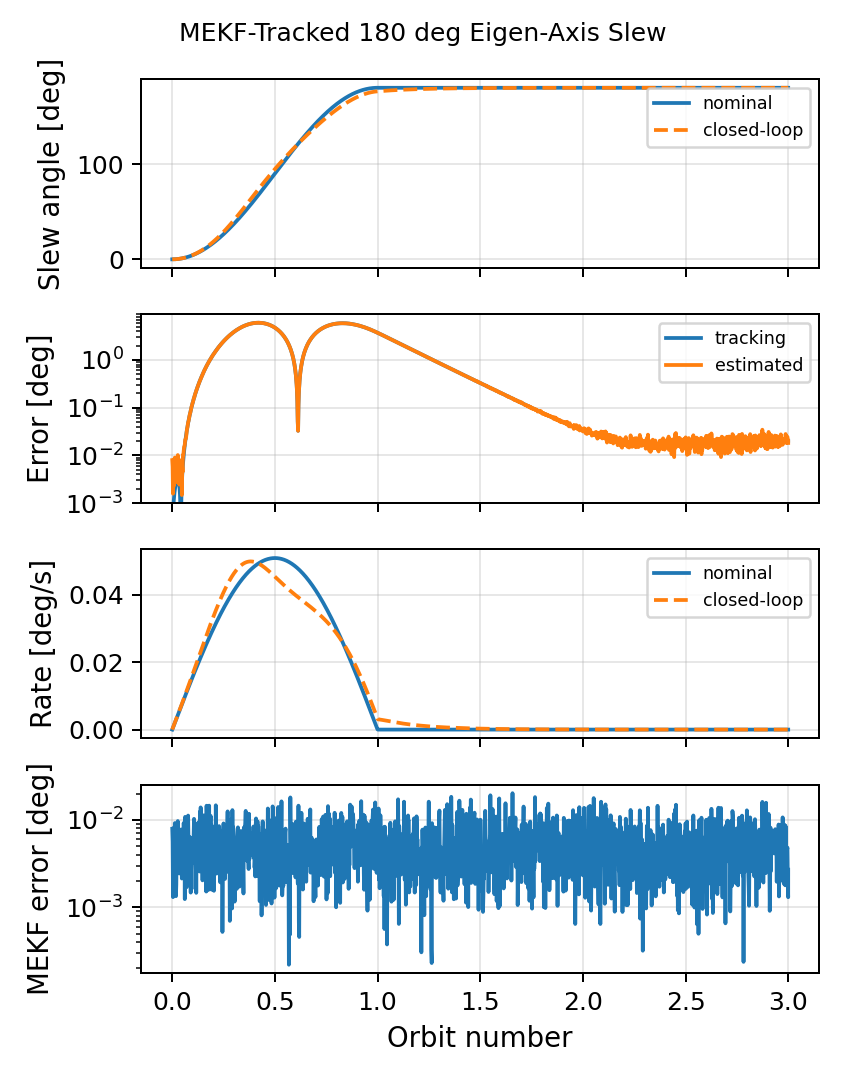
\includegraphics[width=\linewidth]{eigen_axis_slew_tracking.png}
\caption{Nominal and closed-loop states for the $180^\circ$ eigen-axis
slew.  The controller uses the HW3 MEKF state estimate; the estimator
error remains small compared with the trajectory-tracking error.}
\label{fig:slew-tracking}
\end{figure}

The actuator commands remain inside the modeled RCS capability
(Fig.~\ref{fig:slew-inputs}).  The largest commanded body torque is
\SI{125.0}{N.m}, the largest achieved torque is
\SI{125.0}{N.m}, and the largest individual thruster command is
\SI{78.7}{N}.  The allocation keeps net force below
\SI{3.3e-2}{N}, so the maneuver is effectively torque-only in the
coupled orbit simulation.  The total absolute thruster impulse,
computed as $\int\sum_i |u_i|\,dt$, is
\SI{6.17e5}{N.s}; this is not a propellant-optimal steering law, only a
bounded inverse-dynamics and feedback test.

\begin{figure}[h]
\centering
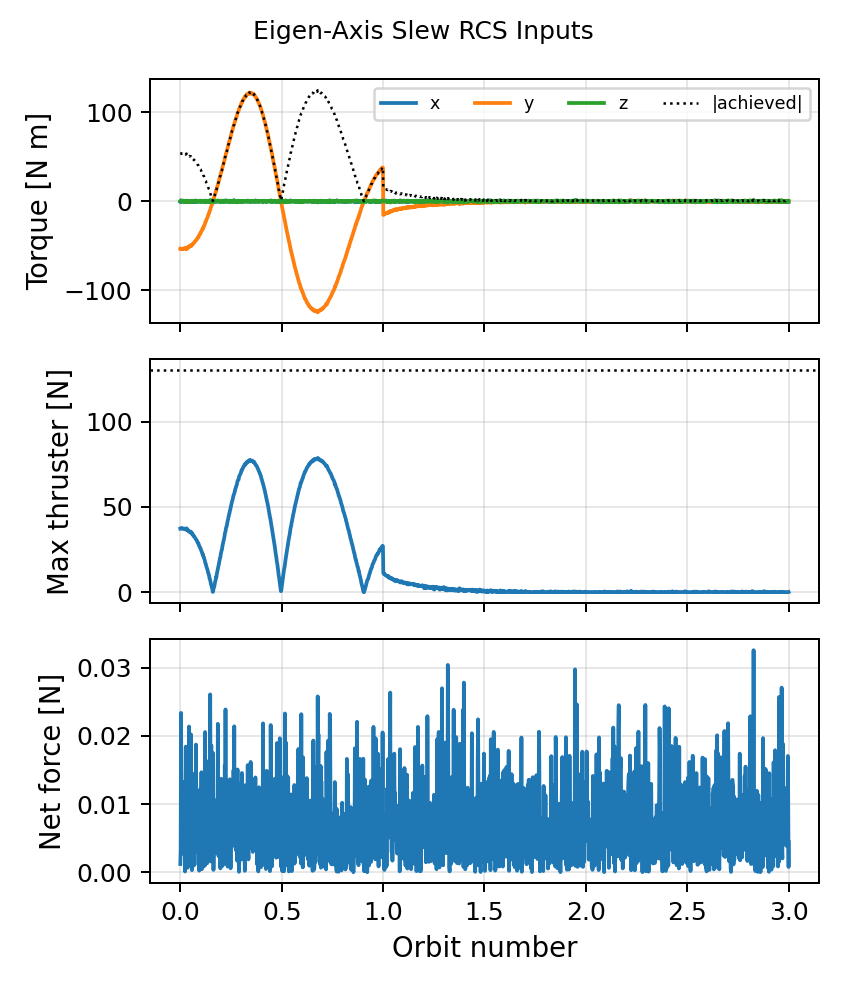
\includegraphics[width=\linewidth]{eigen_axis_slew_inputs.png}
\caption{RCS torque and force commands during the eigen-axis slew.  The
dotted line in the middle panel is the \SI{130}{N} per-thruster limit.}
\label{fig:slew-inputs}
\end{figure}

\subsection{Comparison With Direct Regulation}

I compared the planned slew against the same LQR feedback law used as a
direct regulator from the identical $180^\circ$ initial attitude
(Fig.~\ref{fig:slew-regulator-compare}).  In this single-axis case the
direct regulator converges slightly faster, settling in
\SI{7430}{s} and ending at \SI{0.0167}{deg} error, because it simply
saturates the pitch torque command near \SI{200}{N.m} and drives toward
the target as fast as the imposed torque limit permits.  It also uses a
larger individual thruster command, \SI{112.8}{N}, and reaches a much
higher rate error, \SI{0.136}{deg/s}, than the planned slew's
\SI{0.0085}{deg/s}.

The practical difference is predictability.  The eigen-axis slew gives
a specified maneuver time, a known rest-to-rest rate profile, and
bounded inverse-dynamics inputs before simulation.  The direct
regulator has no planned rate or torque history; for a far initial
condition it behaves like a saturated nonlinear controller.  It works
for this pitch-axis test because the attitude-log error selects the
right rotation axis and the RCS torque limit is high enough, but it
does not by itself guarantee actuator-feasible motion for arbitrary
large-angle slews.

\begin{figure}[h]
\centering
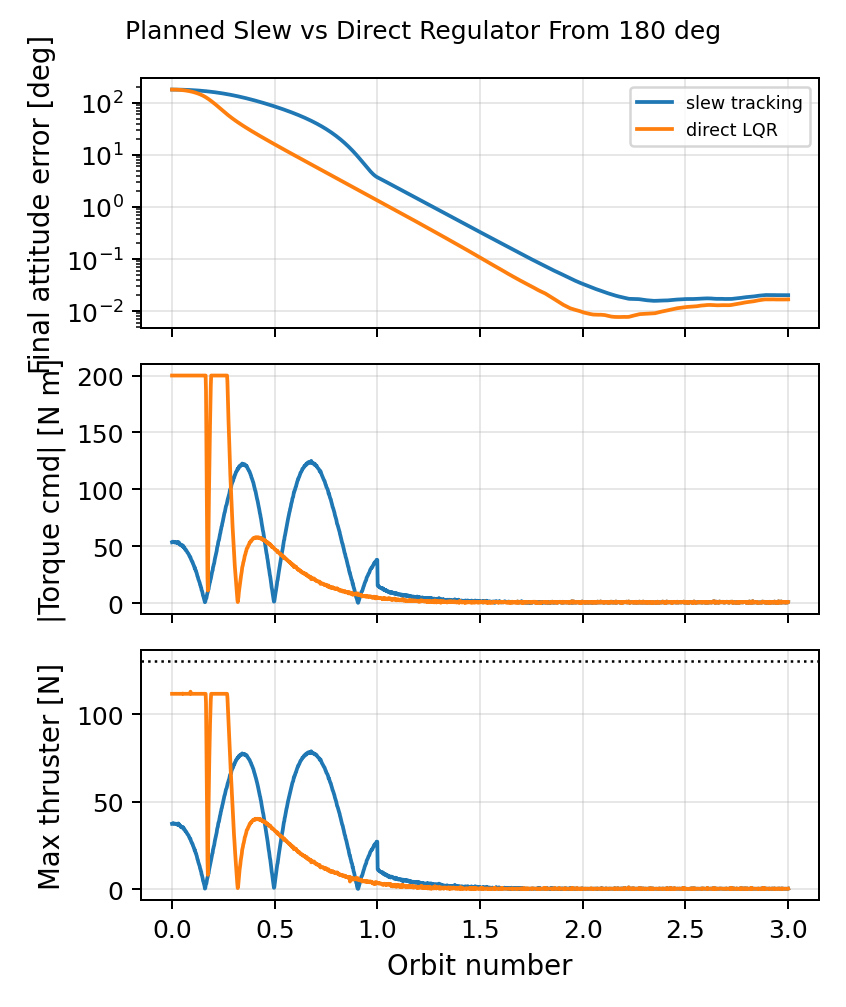
\includegraphics[width=\linewidth]{eigen_axis_slew_regulator_compare.png}
\caption{Comparison between the planned eigen-axis slew and a direct
LQR regulator from the same $180^\circ$ initial attitude.  The direct
regulator is faster here, but only by saturating the torque command and
using higher rates.}
\label{fig:slew-regulator-compare}
\end{figure}

% ==================================================================
\begin{thebibliography}{9}

\bibitem{wie2008}
B.~Wie,
\textit{Space Vehicle Dynamics and Control}, 2nd ed.
AIAA Education Series, 2008. Chapter 7.

\bibitem{bedrossian2009}
N.~Bedrossian, S.~Bhatt, M.~Lebsock, and E.~Wong,
``International Space Station zero-propellant maneuver,''
\textit{Journal of Guidance, Control, and Dynamics},
vol.~32, no.~4, pp.~1193--1201, 2009.

\bibitem{hondatasheet}
Honeywell Defense and Space,
``M1000 Control Moment Gyroscope,'' product information sheet.

\bibitem{nasa_iss_prop}
NASA, ``International Space Station Propulsion System,''
ISS Familiarization Manual, ISS FAM C TD9702A, 1998.

\bibitem{manchester_l16}
Z.~Manchester,
``Lecture 16: Attitude regulation and slew maneuvers,''
Spacecraft Attitude Dynamics and Control lecture notes, 2026.
Available: \url{https://github.com/zacmanchester/spacecraft-attitude-course/blob/main/lecture%20notes/Lecture%2016/Lecture%2016.pdf}

\end{thebibliography}

\end{document}
